\documentclass[tikz, border=10pt]{standalone}
\usepackage{tikz}
\usetikzlibrary{shapes, positioning, matrix, shadows}

\begin{document}
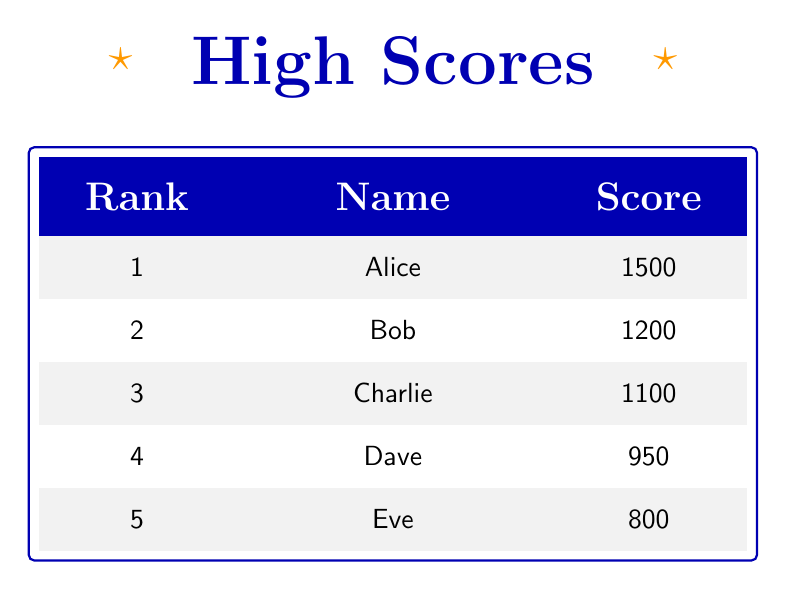
\begin{tikzpicture}[
    font=\sffamily,
    header/.style={
        fill=blue!70!black,
        text=white,
        font=\Large\bfseries,
        minimum height=1cm,
        minimum width=2.5cm
    },
    row_odd/.style={
        fill=gray!10,
        minimum height=0.8cm,
        minimum width=2.5cm
    },
    row_even/.style={
        fill=white,
        minimum height=0.8cm,
        minimum width=2.5cm
    },
    title/.style={
        font=\Huge\bfseries\color{blue!70!black},
        align=center
    }
]

    % Title
    \node[title] (title) at (0, 1.5) {High Scores};

    % Matrix for the table
    \matrix (scores) [
        matrix of nodes,
        nodes={draw=none, anchor=center},
        column sep=0pt,
        row sep=0pt,
        below=0.5cm of title
    ] {
        |[header]| Rank & |[header, minimum width=4cm]| Name & |[header]| Score \\
        |[row_odd]| 1 & |[row_odd, minimum width=4cm]| Alice & |[row_odd]| 1500 \\
        |[row_even]| 2 & |[row_even, minimum width=4cm]| Bob & |[row_even]| 1200 \\
        |[row_odd]| 3 & |[row_odd, minimum width=4cm]| Charlie & |[row_odd]| 1100 \\
        |[row_even]| 4 & |[row_even, minimum width=4cm]| Dave & |[row_even]| 950 \\
        |[row_odd]| 5 & |[row_odd, minimum width=4cm]| Eve & |[row_odd]| 800 \\
    };

    % Border for the table
    \draw[thick, blue!70!black, rounded corners=2pt] (scores.north west) rectangle (scores.south east);
    
    % Trophy icon (simplified)
    \node[right=0.5cm of title, yshift=0.1cm, text=orange!80!yellow, font=\LARGE] {$\star$}; 
    \node[left=0.5cm of title, yshift=0.1cm, text=orange!80!yellow, font=\LARGE] {$\star$};

\end{tikzpicture}
\end{document}
